\chapter{Euler's Method}

How do computers approximate the solution to a differential equation that 
cannot be explicitly solved? Let's consider the differential equation 
$$\frac{dy}{dx} = x + y \text{ with initial condition } y(0) = 1$$

This means the solution passes through the point (0, 1). Additionally, the 
slope of the solution is $\frac{dy}{dx} = 0 + 1 = 1$ at that point. This means 
we can approximate the solution with the linear function $L(x) = x + 1$ (see 
figure \ref{fig:euler1}). As you can see, near $(0,1)$ the approximation is 
good, but as $x$ increases, the divergence between the actual solution and the 
approximation grows. 

\begin{figure}[htbp]
\centering
\begin{tikzpicture}
    \begin{axis}[xmin = -0.1, xmax = 1.2, xtick = {1}, ymin = -0.3, ymax = 5, 
    ytick = {1}, axis lines = center, xlabel = $x$, ylabel = $y$]
    \addplot[red, domain = 0:1]{-1*x + 2*e^x - 1};
    \addplot[blue, thick, domain = 0:1]{x + 1};
    \node[red] at (0.5, 3) {solution curve};
    \node[blue] at (0.75, 0.9) {$L(x)$};
    \end{axis}
\end{tikzpicture}
\caption{A first Euler approximation}
\label{fig:euler1}
\end{figure}

How can we make a better approximation? Suppose we stop the first 
approximation at $x = 1.5$, re-evaluate $\frac{dy}{dx}$, and use that to make 
a second linear approximation. When $x = 0.5$, $L(x) = 0.5 + 1 = 1.5$. Taking 
the point $(0.5, 1.5)$, then $\frac{dy}{dx} = 0.5 + 1.5 = 2$. Then we can 
write a second linear approximation, $L_2(x) = 2(x - 0.5) + 1.5 = 2x - 1 + 1.5 
= 2x + 0.5$ As you can see (figure \ref{fig:euler2}), this new approximation 
is closer than our first approximation. We call this an approximation with a 
step size of 0.5.

\begin{figure}[htbp]
\centering
\begin{tikzpicture}
    \begin{axis}[xmin = -0.1, xmax = 1.2, xtick = {1}, ymin = -0.3, ymax = 5, 
    ytick = {1}, axis lines = center, xlabel = $x$, ylabel = $y$]
    \addplot[red, domain = 0:1]{-1*x + 2*e^x - 1};
    \addplot[blue, thick, domain = 0:0.5]{x + 1};
    \addplot[blue, thick, domain = 0.5:1]{2*x + 0.5};
    \draw[black, dashed](0.5, 0) -- (0.5, 1.5);
    \node[red] at (0.5, 3) {solution curve};
    \node[blue] at (0.25, 0.9) {$L(x)$};
    \node[blue] at (0.75, 1) {$L_2(x)$};
    \end{axis}
\end{tikzpicture}
\caption{An Euler approximation with step size 0.5}
\label{fig:euler2}
\end{figure}

We can improve this further by taking a step size of 0.25 (see figure 
\ref{fig:euler3}). As the step size decreases and the step number increases, 
the approximation gets closer and closer to the true solution. 

\begin{figure}[htbp]
\centering
\begin{tikzpicture}
    \begin{axis}[xmin = -0.1, xmax = 1.2, xtick = {1}, ymin = -0.3, ymax = 5, 
    ytick = {1}, axis lines = center, xlabel = $x$, ylabel = $y$]
    \addplot[red, domain = 0:1]{-1*x + 2*e^x - 1};
    \addplot[blue, thick, domain = 0:0.25]{x + 1};
    \addplot[mark=*, blue](0.25, 1.25);
    \addplot[blue, thick, domain = 0.25:0.5]{1.5*(x - 0.25) + 1.25};
    \addplot[mark=*, blue](0.5, 1.625);
    \addplot[blue, thick, domain = 0.5:0.75]{2.125*(x - 0.5) + 1.625};
    \addplot[mark=*, blue](0.75, 2.15625);
    \addplot[blue, thick, domain = 0.75:1]{2.90625*(x - 0.75) + 2.15625};
    \addplot[mark=*, blue](1, 2.88281);
    \end{axis}
\end{tikzpicture}
\caption{An Euler approximation with step size 0.25}
\label{fig:euler3}
\end{figure}

In general, Euler's method is a numerical process similar to sketching a 
solution on a slope field. One begins at the given initial value, proceeds for 
a short step in the direction indicated by the slope field. You adjust the 
slope of your approximation based on the value of the slope field at the end 
of each step. 

For a first-order differential equation, let $\frac{dy}{dx} = F(x, y)$ and 
$y(x_0) = y_0$. If we have step size $h$, then our successive $x$-values are 
$x_1 = x_0 + h$, $x_2 = x_1 + h$, etc. The differential equation tells us that 
the slope at $x_0$ is $F(x_0, y_0)$. Then $y_1 = y_0 + hF(x_0, y_0)$ (see 
figure \ref{fig:eulervis}). 

\begin{figure}[htbp]
\centering
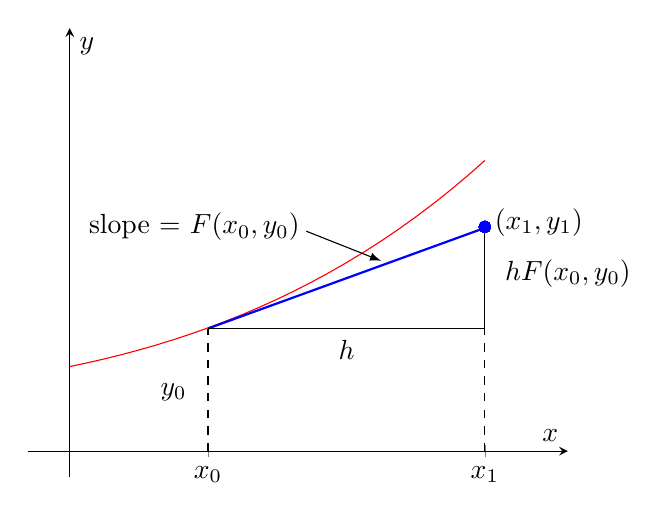
\begin{tikzpicture}
    \begin{axis}[xmin = -0.1, xmax = 1.2, xtick = {0.333, 1}, xticklabels = 
    {$x_0$, $x_1$}, ymin = -0.3, ymax = 5, ytick = \empty, axis lines = center, 
    xlabel = $x$, ylabel = $y$, clip = false]
    \addplot[red, domain = 0:1]{-1*x + 2*e^x - 1};
    \addplot[blue, thick, domain = 0.333:1]{(0.333 + 1.45)*(x - 0.333) + 1.45};
    \draw[black, dashed](0.333, 0) -- (0.333, 1.45);
    \draw[black, dashed] (1, 0) -- (1, 2.651);
    \draw[black] (0.333, 1.45) -- (1, 1.45);
    \draw[black] (1, 1.45) -- (1, 2.651);
    \addplot[mark=*, blue](1, 2.651);
    \node[] at (0.25, 0.7) {$y_0$};
    \node[] at (0.667, 1.2) {$h$};
    \node[] at (1.2, 2.1) {$hF(x_0, y_0)$};
    \node[] at (1.13, 2.7) {$(x_1, y_1)$};
    \node[] at (0.3, 2.65) {slope = $F(x_0, y_0)$};
    \draw[-latex](0.57, 2.6) -- (0.75, 2.25);
    \end{axis}
\end{tikzpicture}
\caption{Visualization of Euler's method}
\label{fig:eulervis}
\end{figure}

Continuing, once we've found $y_1$, we can then define $x_2 = x_1 + h$ and 
$y_2 = y_1 + hF(x_1, y_1)$. And in general, for an initial-value problem when 
$\frac{dy}{dx} = F(x, y)$ and $y(x_0) = y_0$, we can make an approximation 
with step size $h$ where:
$$y_n = y_{n-1} + hF(x_{n-1},y_{n-1})$$
where $n = 1, 2, 3, \cdots$. 

\textbf{Example}: Use Euler's method with a step size of 0.2 to approximate 
the value of $y(1)$ if $\frac{dy}{dx} = 2x + y$ and $y(0) = 1$. 

\textbf{Solution}: We are given $h = 0.2$, $x_0 = 0$, $y_0 = 1$, and $F(x, y) 
= 2x + y$. This means we will need 10 steps to reach $x_{5} = 1$. So we know 
that:
$$y_1 = 1 + 0.2[2(0) + 1] = 1 + 0.2[1] = 1.2$$
$$y_2 = 1.2 + 0.2[2(0.2) + 1.2] = 1.2 + 0.2(1.6) = 1.52$$
$$y_3 = 1.52 + 0.2[2(0.4) + 1.52] = 1.984$$

We can continue in this manner. The results are shown in the table:
\begin{center}
\begin{tabular}{|c|c|c|c|}\hline
n & $x_n$ & $y_n$ & $F(x_n, y_n)$ \\\hline
0 & 0 & 1 & 1\\\hline
1 & 0.2 & 1.2 & 1.6\\\hline
2 & 0.4 & 1.52 & 2.32\\\hline
3 & 0.6 & 1.984 & 3.184\\\hline
4 & 0.8 & 2.6208 & 4.2208\\\hline
5 & 1 & 3.46496 & --\\\hline
\end{tabular}
\end{center}

Therefore, $y(1) \approx 3.4696$.